\documentclass{standalone}
\usepackage{tikz}
\usetikzlibrary{patterns, positioning}


\begin{document}
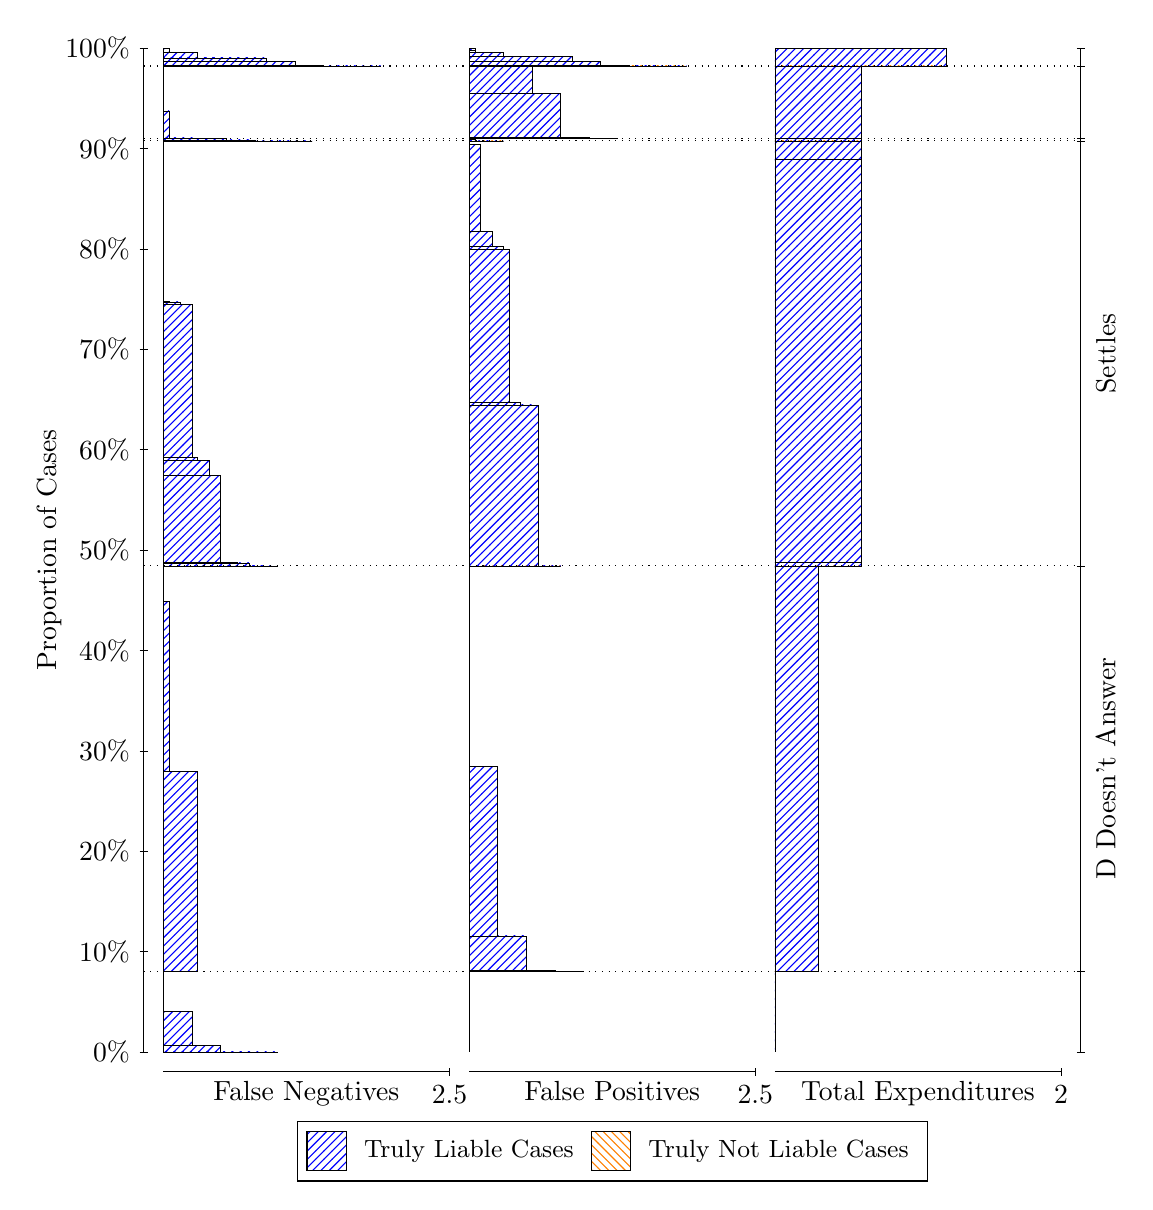
\begin{tikzpicture}
\draw[black, very thin] (1.5,1.75) -- (1.5,14.5);
\node[rotate=90, text=black, anchor=center] at (0.3, 8.125) {Proportion of Cases};
\draw[black, very thin] (1.45,1.75) -- (1.55,1.75);
\node[text=black, anchor=east] at (1.45, 1.75) {0\%};
\draw[black, very thin] (1.45,3.025) -- (1.55,3.025);
\node[text=black, anchor=east] at (1.45, 3.025) {10\%};
\draw[black, very thin] (1.45,4.3) -- (1.55,4.3);
\node[text=black, anchor=east] at (1.45, 4.3) {20\%};
\draw[black, very thin] (1.45,5.575) -- (1.55,5.575);
\node[text=black, anchor=east] at (1.45, 5.575) {30\%};
\draw[black, very thin] (1.45,6.85) -- (1.55,6.85);
\node[text=black, anchor=east] at (1.45, 6.85) {40\%};
\draw[black, very thin] (1.45,8.125) -- (1.55,8.125);
\node[text=black, anchor=east] at (1.45, 8.125) {50\%};
\draw[black, very thin] (1.45,9.4) -- (1.55,9.4);
\node[text=black, anchor=east] at (1.45, 9.4) {60\%};
\draw[black, very thin] (1.45,10.675) -- (1.55,10.675);
\node[text=black, anchor=east] at (1.45, 10.675) {70\%};
\draw[black, very thin] (1.45,11.95) -- (1.55,11.95);
\node[text=black, anchor=east] at (1.45, 11.95) {80\%};
\draw[black, very thin] (1.45,13.225) -- (1.55,13.225);
\node[text=black, anchor=east] at (1.45, 13.225) {90\%};
\draw[black, very thin] (1.45,14.5) -- (1.55,14.5);
\node[text=black, anchor=east] at (1.45, 14.5) {100\%};

\draw[black, very thin] (13.4,1.75) -- (13.4,14.5);
\draw[black, very thin] (13.35,1.75) -- (13.45,1.75);
\node[anchor=west] at (13.35, 1.75) {};
\draw[black, very thin] (13.35,2.7698) -- (13.45,2.7698);
\node[anchor=west] at (13.35, 2.7698) {};
\draw[black, very thin] (13.35,7.9242) -- (13.45,7.9242);
\node[anchor=west] at (13.35, 7.9242) {};
\draw[black, very thin] (13.35,13.321) -- (13.45,13.321);
\node[anchor=west] at (13.35, 13.321) {};
\draw[black, very thin] (13.35,13.354) -- (13.45,13.354);
\node[anchor=west] at (13.35, 13.354) {};
\draw[black, very thin] (13.35,14.272) -- (13.45,14.272);
\node[anchor=west] at (13.35, 14.272) {};
\draw[black, very thin] (13.35,14.5) -- (13.45,14.5);
\node[anchor=west] at (13.35, 14.5) {};

\draw[black, very thin, pattern color=blue, pattern=north east lines] (1.75,1.75) rectangle (3.2033,1.75);
\draw[black, very thin, pattern color=blue, pattern=north east lines] (1.75,1.75) rectangle (2.84,1.7507);
\draw[black, very thin, pattern color=blue, pattern=north east lines] (1.75,1.7507) rectangle (2.4767,1.8316);
\draw[black, very thin, pattern color=blue, pattern=north east lines] (1.75,1.8316) rectangle (2.1133,2.2606);
\draw[black, very thin, pattern color=orange, pattern=north west lines] (1.75,2.2606) rectangle (1.75,2.2606);
\draw[black, very thin, pattern color=blue, pattern=north east lines] (1.75,2.2606) rectangle (1.75,2.7698);
\draw[black, very thin, pattern color=blue, pattern=north east lines] (1.75,2.7698) rectangle (2.186,5.3157);
\draw[black, very thin, pattern color=blue, pattern=north east lines] (1.75,5.3157) rectangle (1.8227,7.471);
\draw[black, very thin, pattern color=orange, pattern=north west lines] (1.75,7.471) rectangle (1.75,7.471);
\draw[black, very thin, pattern color=blue, pattern=north east lines] (1.75,7.471) rectangle (1.75,7.9242);
\draw[black, very thin, pattern color=blue, pattern=north east lines] (1.75,7.9242) rectangle (3.2033,7.9242);
\draw[black, very thin, pattern color=blue, pattern=north east lines] (1.75,7.9242) rectangle (3.058,7.9242);
\draw[black, very thin, pattern color=blue, pattern=north east lines] (1.75,7.9242) rectangle (2.9127,7.9242);
\draw[black, very thin, pattern color=blue, pattern=north east lines] (1.75,7.9242) rectangle (2.84,7.9603);
\draw[black, very thin, pattern color=blue, pattern=north east lines] (1.75,7.9603) rectangle (2.6947,7.9697);
\draw[black, very thin, pattern color=blue, pattern=north east lines] (1.75,7.9697) rectangle (2.5493,7.9712);
\draw[black, very thin, pattern color=blue, pattern=north east lines] (1.75,7.9712) rectangle (2.4767,9.0732);
\draw[black, very thin, pattern color=blue, pattern=north east lines] (1.75,9.0732) rectangle (2.3313,9.2679);
\draw[black, very thin, pattern color=blue, pattern=north east lines] (1.75,9.2679) rectangle (2.186,9.3006);
\draw[black, very thin, pattern color=blue, pattern=north east lines] (1.75,9.3006) rectangle (2.1133,11.248);
\draw[black, very thin, pattern color=blue, pattern=north east lines] (1.75,11.248) rectangle (1.968,11.277);
\draw[black, very thin, pattern color=blue, pattern=north east lines] (1.75,11.277) rectangle (1.8227,11.282);
\draw[black, very thin, pattern color=orange, pattern=north west lines] (1.75,11.282) rectangle (1.75,11.282);
\draw[black, very thin, pattern color=blue, pattern=north east lines] (1.75,11.282) rectangle (1.75,13.321);
\draw[black, very thin, pattern color=blue, pattern=north east lines] (1.75,13.321) rectangle (3.6393,13.321);
\draw[black, very thin, pattern color=blue, pattern=north east lines] (1.75,13.321) rectangle (3.276,13.321);
\draw[black, very thin, pattern color=blue, pattern=north east lines] (1.75,13.321) rectangle (2.9127,13.332);
\draw[black, very thin, pattern color=blue, pattern=north east lines] (1.75,13.332) rectangle (2.5493,13.353);
\draw[black, very thin, pattern color=blue, pattern=north east lines] (1.75,13.353) rectangle (2.186,13.354);
\draw[black, very thin, pattern color=orange, pattern=north west lines] (1.75,13.354) rectangle (1.75,13.354);
\draw[black, very thin, pattern color=blue, pattern=north east lines] (1.75,13.354) rectangle (2.186,13.358);
\draw[black, very thin, pattern color=blue, pattern=north east lines] (1.75,13.358) rectangle (1.8227,13.701);
\draw[black, very thin, pattern color=orange, pattern=north west lines] (1.75,13.701) rectangle (1.75,13.701);
\draw[black, very thin, pattern color=blue, pattern=north east lines] (1.75,13.701) rectangle (1.75,14.272);
\draw[black, very thin, pattern color=blue, pattern=north east lines] (1.75,14.272) rectangle (4.5113,14.272);
\draw[black, very thin, pattern color=blue, pattern=north east lines] (1.75,14.272) rectangle (4.148,14.272);
\draw[black, very thin, pattern color=blue, pattern=north east lines] (1.75,14.272) rectangle (3.7847,14.275);
\draw[black, very thin, pattern color=blue, pattern=north east lines] (1.75,14.275) rectangle (3.4213,14.326);
\draw[black, very thin, pattern color=blue, pattern=north east lines] (1.75,14.326) rectangle (3.276,14.326);
\draw[black, very thin, pattern color=blue, pattern=north east lines] (1.75,14.326) rectangle (3.058,14.374);
\draw[black, very thin, pattern color=blue, pattern=north east lines] (1.75,14.374) rectangle (2.9127,14.374);
\draw[black, very thin, pattern color=blue, pattern=north east lines] (1.75,14.374) rectangle (2.6947,14.374);
\draw[black, very thin, pattern color=blue, pattern=north east lines] (1.75,14.374) rectangle (2.5493,14.375);
\draw[black, very thin, pattern color=blue, pattern=north east lines] (1.75,14.375) rectangle (2.3313,14.375);
\draw[black, very thin, pattern color=blue, pattern=north east lines] (1.75,14.375) rectangle (2.186,14.375);
\draw[black, very thin, pattern color=blue, pattern=north east lines] (1.75,14.375) rectangle (2.186,14.442);
\draw[black, very thin, pattern color=blue, pattern=north east lines] (1.75,14.442) rectangle (1.8227,14.443);
\draw[black, very thin, pattern color=blue, pattern=north east lines] (1.75,14.443) rectangle (1.8227,14.495);
\draw[black, very thin, pattern color=orange, pattern=north west lines] (1.75,14.495) rectangle (1.75,14.495);
\draw[black, very thin, pattern color=blue, pattern=north east lines] (1.75,14.495) rectangle (1.75,14.5);
\draw[black, very thin, pattern color=orange, pattern=north west lines] (5.6333,1.75) rectangle (5.6333,1.75);
\draw[black, very thin, pattern color=blue, pattern=north east lines] (5.6333,1.75) rectangle (5.6333,2.7698);
\draw[black, very thin, pattern color=orange, pattern=north west lines] (5.6333,2.7698) rectangle (7.0867,2.7698);
\draw[black, very thin, pattern color=blue, pattern=north east lines] (5.6333,2.7698) rectangle (7.0867,2.7699);
\draw[black, very thin, pattern color=blue, pattern=north east lines] (5.6333,2.7699) rectangle (6.7233,2.7837);
\draw[black, very thin, pattern color=blue, pattern=north east lines] (5.6333,2.7837) rectangle (6.36,3.223);
\draw[black, very thin, pattern color=blue, pattern=north east lines] (5.6333,3.223) rectangle (5.9967,5.3783);
\draw[black, very thin, pattern color=blue, pattern=north east lines] (5.6333,5.3783) rectangle (5.6333,7.9242);
\draw[black, very thin, pattern color=orange, pattern=north west lines] (5.6333,7.9242) rectangle (6.796,7.9242);
\draw[black, very thin, pattern color=blue, pattern=north east lines] (5.6333,7.9242) rectangle (6.796,7.9242);
\draw[black, very thin, pattern color=orange, pattern=north west lines] (5.6333,7.9242) rectangle (6.6507,7.9242);
\draw[black, very thin, pattern color=blue, pattern=north east lines] (5.6333,7.9242) rectangle (6.6507,7.9243);
\draw[black, very thin, pattern color=orange, pattern=north west lines] (5.6333,7.9243) rectangle (6.5053,7.9243);
\draw[black, very thin, pattern color=blue, pattern=north east lines] (5.6333,7.9243) rectangle (6.5053,9.9632);
\draw[black, very thin, pattern color=blue, pattern=north east lines] (5.6333,9.9632) rectangle (6.4327,9.9681);
\draw[black, very thin, pattern color=blue, pattern=north east lines] (5.6333,9.9681) rectangle (6.2873,9.9972);
\draw[black, very thin, pattern color=blue, pattern=north east lines] (5.6333,9.9972) rectangle (6.142,11.944);
\draw[black, very thin, pattern color=blue, pattern=north east lines] (5.6333,11.944) rectangle (6.0693,11.977);
\draw[black, very thin, pattern color=blue, pattern=north east lines] (5.6333,11.977) rectangle (5.924,12.172);
\draw[black, very thin, pattern color=blue, pattern=north east lines] (5.6333,12.172) rectangle (5.7787,13.274);
\draw[black, very thin, pattern color=blue, pattern=north east lines] (5.6333,13.274) rectangle (5.706,13.275);
\draw[black, very thin, pattern color=blue, pattern=north east lines] (5.6333,13.275) rectangle (5.6333,13.321);
\draw[black, very thin, pattern color=orange, pattern=north west lines] (5.6333,13.321) rectangle (6.0693,13.321);
\draw[black, very thin, pattern color=blue, pattern=north east lines] (5.6333,13.321) rectangle (6.0693,13.321);
\draw[black, very thin, pattern color=blue, pattern=north east lines] (5.6333,13.321) rectangle (5.706,13.342);
\draw[black, very thin, pattern color=blue, pattern=north east lines] (5.6333,13.342) rectangle (5.6333,13.354);
\draw[black, very thin, pattern color=orange, pattern=north west lines] (5.6333,13.354) rectangle (7.5227,13.354);
\draw[black, very thin, pattern color=blue, pattern=north east lines] (5.6333,13.354) rectangle (7.5227,13.354);
\draw[black, very thin, pattern color=blue, pattern=north east lines] (5.6333,13.354) rectangle (7.1593,13.369);
\draw[black, very thin, pattern color=blue, pattern=north east lines] (5.6333,13.369) rectangle (6.796,13.924);
\draw[black, very thin, pattern color=blue, pattern=north east lines] (5.6333,13.924) rectangle (6.4327,14.268);
\draw[black, very thin, pattern color=blue, pattern=north east lines] (5.6333,14.268) rectangle (6.0693,14.272);
\draw[black, very thin, pattern color=orange, pattern=north west lines] (5.6333,14.272) rectangle (8.3947,14.272);
\draw[black, very thin, pattern color=blue, pattern=north east lines] (5.6333,14.272) rectangle (8.3947,14.272);
\draw[black, very thin, pattern color=orange, pattern=north west lines] (5.6333,14.272) rectangle (8.0313,14.272);
\draw[black, very thin, pattern color=blue, pattern=north east lines] (5.6333,14.272) rectangle (8.0313,14.272);
\draw[black, very thin, pattern color=orange, pattern=north west lines] (5.6333,14.272) rectangle (7.668,14.272);
\draw[black, very thin, pattern color=blue, pattern=north east lines] (5.6333,14.272) rectangle (7.668,14.277);
\draw[black, very thin, pattern color=orange, pattern=north west lines] (5.6333,14.277) rectangle (7.3047,14.277);
\draw[black, very thin, pattern color=blue, pattern=north east lines] (5.6333,14.277) rectangle (7.3047,14.33);
\draw[black, very thin, pattern color=blue, pattern=north east lines] (5.6333,14.33) rectangle (6.9413,14.396);
\draw[black, very thin, pattern color=orange, pattern=north west lines] (5.6333,14.396) rectangle (6.796,14.396);
\draw[black, very thin, pattern color=blue, pattern=north east lines] (5.6333,14.396) rectangle (6.796,14.396);
\draw[black, very thin, pattern color=blue, pattern=north east lines] (5.6333,14.396) rectangle (6.578,14.398);
\draw[black, very thin, pattern color=orange, pattern=north west lines] (5.6333,14.398) rectangle (6.4327,14.398);
\draw[black, very thin, pattern color=blue, pattern=north east lines] (5.6333,14.398) rectangle (6.4327,14.398);
\draw[black, very thin, pattern color=blue, pattern=north east lines] (5.6333,14.398) rectangle (6.2147,14.398);
\draw[black, very thin, pattern color=blue, pattern=north east lines] (5.6333,14.398) rectangle (6.0693,14.445);
\draw[black, very thin, pattern color=orange, pattern=north west lines] (5.6333,14.445) rectangle (6.0693,14.445);
\draw[black, very thin, pattern color=blue, pattern=north east lines] (5.6333,14.445) rectangle (6.0693,14.446);
\draw[black, very thin, pattern color=blue, pattern=north east lines] (5.6333,14.446) rectangle (5.8513,14.446);
\draw[black, very thin, pattern color=blue, pattern=north east lines] (5.6333,14.446) rectangle (5.706,14.476);
\draw[black, very thin, pattern color=blue, pattern=north east lines] (5.6333,14.476) rectangle (5.706,14.497);
\draw[black, very thin, pattern color=blue, pattern=north east lines] (5.6333,14.497) rectangle (5.6333,14.5);
\draw[black, very thin, pattern color=orange, pattern=north west lines] (9.5167,1.75) rectangle (9.5167,1.75);
\draw[black, very thin, pattern color=blue, pattern=north east lines] (9.5167,1.75) rectangle (9.5167,2.7698);
\draw[black, very thin, pattern color=orange, pattern=north west lines] (9.5167,2.7698) rectangle (10.062,2.7698);
\draw[black, very thin, pattern color=blue, pattern=north east lines] (9.5167,2.7698) rectangle (10.062,7.9242);
\draw[black, very thin, pattern color=orange, pattern=north west lines] (9.5167,7.9242) rectangle (10.607,7.9242);
\draw[black, very thin, pattern color=blue, pattern=north east lines] (9.5167,7.9242) rectangle (10.607,7.9634);
\draw[black, very thin, pattern color=orange, pattern=north west lines] (9.5167,7.9634) rectangle (10.607,7.9634);
\draw[black, very thin, pattern color=blue, pattern=north east lines] (9.5167,7.9634) rectangle (10.607,13.088);
\draw[black, very thin, pattern color=orange, pattern=north west lines] (9.5167,13.088) rectangle (10.607,13.088);
\draw[black, very thin, pattern color=blue, pattern=north east lines] (9.5167,13.088) rectangle (10.607,13.321);
\draw[black, very thin, pattern color=orange, pattern=north west lines] (9.5167,13.321) rectangle (10.607,13.321);
\draw[black, very thin, pattern color=blue, pattern=north east lines] (9.5167,13.321) rectangle (10.607,13.354);
\draw[black, very thin, pattern color=orange, pattern=north west lines] (9.5167,13.354) rectangle (10.607,13.354);
\draw[black, very thin, pattern color=blue, pattern=north east lines] (9.5167,13.354) rectangle (10.607,14.272);
\draw[black, very thin, pattern color=orange, pattern=north west lines] (9.5167,14.272) rectangle (11.697,14.272);
\draw[black, very thin, pattern color=blue, pattern=north east lines] (9.5167,14.272) rectangle (11.697,14.5);
\draw[black, dotted] (1.5,2.7698) -- (13.4,2.7698);
\draw[black, dotted] (1.5,7.9242) -- (13.4,7.9242);
\draw[black, dotted] (1.5,13.321) -- (13.4,13.321);
\draw[black, dotted] (1.5,13.354) -- (13.4,13.354);
\draw[black, dotted] (1.5,14.272) -- (13.4,14.272);
\draw[black, very thin] (1.75,1.5) -- (5.3833,1.5);
\node[text=black, anchor=north] at (3.5667, 1.5) {False Negatives};
\draw[black, very thin] (5.3833,1.45) -- (5.3833,1.55);
\node[text=black, anchor=north] at (5.3833, 1.45) {2.5};

\draw[black, very thin] (5.6333,1.5) -- (9.2667,1.5);
\node[text=black, anchor=north] at (7.45, 1.5) {False Positives};
\draw[black, very thin] (9.2667,1.45) -- (9.2667,1.55);
\node[text=black, anchor=north] at (9.2667, 1.45) {2.5};

\draw[black, very thin] (9.5167,1.5) -- (13.15,1.5);
\node[text=black, anchor=north] at (11.333, 1.5) {Total Expenditures};
\draw[black, very thin] (13.15,1.45) -- (13.15,1.55);
\node[text=black, anchor=north] at (13.15, 1.45) {2};


\node[text=black, centered, rotate=90] at (13.72, 5.347) {D Doesn't Answer};
\node[text=black, centered, rotate=90] at (13.72, 10.622) {Settles};




\draw (7.449999999999999,1.5) node[draw=none] (baseCoordinate) {};
\begin{scope}[align=center]
        \matrix[scale=0.5, draw=black, below=0.5cm of baseCoordinate, nodes={draw}, column sep=0.1cm]{
            \node[rectangle, draw, minimum width=0.5cm, minimum height=0.5cm, pattern color=blue, pattern=north east lines] {}; &
            \node[draw=none, font=\small, text=black] (B) {Truly Liable Cases}; &
            \node[rectangle, draw, minimum width=0.5cm, minimum height=0.5cm, pattern color=orange, pattern=north west lines] {}; &
            \node[draw=none, font=\small, text=black] (B) {Truly Not Liable Cases}; \\
            };
\end{scope}

\end{tikzpicture}
\end{document}